% exactness-slow-walk.tex --- Appendix D.1's proofs at reading pace: the slow walk the thesis points to from Appendix D.1, restating D.1.1's seven statements and the exactness table locally, so that every Theorem, Lemma, Corollary and Table reference below resolves on these pages; a thesis section, figure or table that is not restated is named by its number.
% Compiles standalone with pdflatex; the one graphic is read from the thesis tree (paper/figures/protocol_doors.pdf) when that file is present, and a described placeholder box stands in when it is not.

\documentclass[11pt,a4paper]{article}

\usepackage[margin=2.6cm]{geometry}
\usepackage{amsmath,amssymb,amsthm,mathtools}
\usepackage{bbm}
\usepackage{booktabs}
\usepackage{graphicx}
\usepackage{float}
\usepackage{microtype}
\usepackage[colorlinks=true,linkcolor=black,urlcolor=black,citecolor=black]{hyperref}

% --- the thesis macros this text uses, as bsc-thesis.tex defines them ---
\DeclareMathOperator{\SO}{SO}
\DeclareMathOperator{\Tr}{Tr}
\newcommand{\C}{\mathbb{C}}
\newcommand{\R}{\mathbb{R}}
\newcommand{\Id}{\mathbbm{1}}
\newcommand{\sigmaz}{\sigma_z}
\newcommand{\sigmavec}{\boldsymbol{\sigma}}
\newcommand{\pmat}[1]{\begin{pmatrix} #1 \end{pmatrix}}
\newcommand{\Tgroup}{\mathcal{T}}
\newcommand{\Ogroup}{\mathcal{O}}
\newcommand{\Igroup}{\mathcal{I}}
\newcommand{\TwoT}{2\Tgroup}
\newcommand{\TwoO}{2\Ogroup}
\newcommand{\TwoI}{2\Igroup}
\newcommand{\phig}{\tau}      % golden ratio, Conway--Smith
\newcommand{\invphig}{\sigma} % its inverse
\newcommand{\ket}[1]{|#1\rangle}
\newcommand{\bra}[1]{\langle#1|}
\newcommand{\braket}[2]{\langle#1|#2\rangle}
\newcommand{\ketbra}[2]{|#1\rangle\langle#2|}
\DeclarePairedDelimiter{\abs}{\lvert}{\rvert}
\newenvironment{sketch}{\renewcommand{\qedsymbol}{}\begin{proof}[Sketch]}{\end{proof}}

\newtheorem{theorem}{Theorem}
\newtheorem{lemma}[theorem]{Lemma}
\newtheorem{corollary}[theorem]{Corollary}

\title{\bfseries Circuits do arithmetic\\[2mm]
\large Appendix D.1's proofs at reading pace}
\author{}
\date{}

\begin{document}
\maketitle
\vspace{-12mm}

\section*{Scope}

This document is the slow walk behind Appendix D.1 of the thesis: the refresher on the ring of the gate sets, the protocol model, the three steps that prove the branch decomposition and the directions corollary, the refresher on what is and is not in $K_\R$ with Lemma~\ref{lem:membership}'s full proof, the rotation-proof witness, the octahedron exhibited, the three doors, the alignment corollary slowly, and the geometric dictionary. The thesis prints the seven statements with proof sketches, the octahedron's exhibition and Theorem~\ref{thm:weight}'s arithmetic; the rest is walked here. It is self-contained: Section~\ref{sec:statements} restates those statements and the exactness table locally with the thesis's own labels, so every \emph{Theorem}, \emph{Lemma} and \emph{Corollary} below refers to a statement printed on these pages; a section, figure or table of the thesis that is not restated is named by its number.

\section{The statements, restated}\label{sec:statements}

The two displays the text below quotes from the thesis's Chapter~2 and Chapter~4. A Platonic solid POVM with $V$ vertices $\{\hat n_k\} \subset \R^3$ on the Bloch sphere has effects
\begin{equation} \label{eq:povmform}
E_k = \frac{2}{V} \ketbra{\psi_k}{\psi_k} = \frac{2}{V} \frac12 \left( \Id + \hat{n}_k \cdot \sigmavec \right),
\end{equation}
and the golden gate and its conjugate are
\begin{equation}\label{eq:golden-gate}
    \Phi = \frac{1}{2} \begin{pmatrix} \phig + i\phig^{-1} & 1 \\ -1 & \phig - i\phig^{-1} \end{pmatrix}, \quad \Phi^\star = \frac{1}{2} \begin{pmatrix} -\invphig - i\invphig^{-1} & 1 \\ -1 & -\invphig + i\invphig^{-1} \end{pmatrix}.
\end{equation}

Throughout, $\mathcal{R} \subset \C$ is a subring containing $i$ and closed under complex conjugation, $K = \operatorname{Frac}\mathcal{R}$ its field of fractions and $K_\R = K \cap \R$ the real subfield. The statements follow, numbered as in the thesis; their footnotes and citations are the thesis's and are not repeated here.

Call a gate set \textit{admissible} if every one of its gates has entries in $\mathcal{R} = \mathbb{Z}[\phig, i, \sqrt{2}, \tfrac{1}{2}]$, whence $K_\R = \mathbb{Q}(\sqrt{2},\sqrt{5})$. Every gate set of this thesis is admissible and contains $\TwoT$: $\TwoT$, Clifford, Clifford${}+T$, $\TwoI$, Clifford${}+\Phi$, and their unions, each adjoined with an entangling Clifford such as CNOT, whose $0$'s and $1$'s cost nothing. A protocol implements a POVM \textit{exactly} if its effects are the POVM's.

\begin{theorem} \label{thm:main}
Over any admissible gate set, of the five Platonic solid POVMs only the octahedral is exactly implementable, i.e., with no approximation, by a protocol in the sense of Lemma~\ref{lem:branch}: the other four in no pose, the octahedron at least in atlas orientation over any set containing $\TwoT$, where its vertices are the Pauli axes. Over any admissible gate set, no deterministic protocol in the sense of Theorem~\ref{thm:weight}, hence no dilation, implements any of the five exactly: the octahedron's exactness costs a coin, a discarded branch, or unbounded repetition.
\end{theorem}

\begin{sketch}
Four impossibilities by arithmetic plus one construction: Lemmas~\ref{lem:witness} and~\ref{lem:membership} with Table~\ref{tab:povm-exactness} put the other four solids' witness outside $K_\R$ in every pose, where Corollary~\ref{cor:directions} bars them, while the octahedron's Pauli axes are realized by a three-word coin from $\TwoT$. For the octahedron, determinism fails separately: by Theorem~\ref{thm:weight}, a deterministic protocol weighs only dyadically, and its effects weigh $\tfrac{1}{3}$.
\end{sketch}

\begin{lemma}[branch decomposition] \label{lem:branch}
Let $\mathcal{R} \subset \C$ contain $i$ and be closed under complex conjugation, let a gate set have all its matrix entries in $\mathcal{R}$, and consider any protocol built from it: one data qubit, finitely many ancillas prepared in $\ket{0}$, gates from the set, computational-basis measurements, classical coins of arbitrary bias, feedforward (later gates conditioned on earlier coins and outcomes), and classical post-processing assigning at most one label per record, a randomized labelling being one more coin. Every effect it realizes decomposes as
\begin{equation*}
E_k \;=\; \sum_{b} p_b \ketbra{a_b}{a_b}, \qquad \ket{a_b} \in \mathcal{R}^2, \quad p_b > 0,
\end{equation*}
one term per \textit{branch} $b$, a branch being one complete record of coin values and measurement outcomes that post-processing labels $k$, with $p_b$ the product of the coin probabilities along $b$. If the protocol tosses no coin, every $p_b = 1$.
\end{lemma}

\begin{sketch}
Condition on a branch and every fork is decided, leaving one definite sequence of gates, $0/1$ projectors and $\ket{0}$ ancillas; composing them only adds, multiplies and conjugates entries, which never leaves $\mathcal{R}$, and the coins contribute no operator at all---only the scalar $p_b$.
\end{sketch}

The lemma has two readings. Its \textit{weights} stay in $\mathcal{R}$ under a deterministic protocol (Theorem~\ref{thm:weight}); its \textit{directions} divide once, and land in $K_\R$ either way. The line between them is the coin, the discarded branch, or unbounded repetition.

% NOTE (notation): the letter $w$ stays out of D.1 --- it already means the quaternion real part (Chapter~2, and the latitude of Appendix~C's section ladder), the Pauli-string weight (Appendix~F), and the gate sequence in the synthesis algorithm. \textit{Weight} names $\Tr[E_k]$ throughout D.1, symbolized at its definition point in Theorem~\ref{thm:weight}; the representative of Step~3 has $\Tr[\ketbra{\psi}{\psi}] = N$. The positive multiple in front of $\ketbra{\psi}{\psi}$ is representative-dependent ($\ket{\psi}$ must stay unnormalized to stay in $\mathcal{R}^2$), so it is called \textit{the multiple} or \textit{the scale} and never a weight; Corollary~\ref{cor:directions} leaves it unconstrained. It carries the letter $c$, defined in that corollary and traced through Steps~2 and~3, where it cancels before the ring argument can run; the effect's weight is then $cN$, and $c \notin \mathcal{R}$ in general even though $cN \in \mathcal{R}$ once the coin is banned. The branch weights $p_b$ are untouched. Use symbols over words for greater mathematical precision and clarity.
\begin{corollary}[directions] \label{cor:directions}
Any rank-$1$ effect such a protocol realizes is $c\ketbra{\psi}{\psi}$ for some $c > 0$ and some $\ket{\psi} \in \mathcal{R}^2$, and its Bloch vector $\hat n$ lies in $K_\R^3$. Neither $c$ nor $p_b$ need lie in $\mathcal{R}$.
\end{corollary}

\begin{sketch}
Rank one forces all the $\ket{a_b}$ parallel, so the effect has one direction over $\mathcal{R}$; its Bloch coordinates divide by $\braket{\psi}{\psi}$ and so land in $K_\R$, which is blind to the weight that division removed.
\end{sketch}

\begin{theorem}[weights] \label{thm:weight}
Call a protocol \textit{deterministic} if it tosses no classical coin, discards no branch, and halts within a bounded number of rounds, every run returning an outcome; feedforward is still allowed. A deterministic protocol realizes only effects whose \textit{weight} $\Tr[E_k]$ lies in $\mathcal{R}$. For $\mathcal{R} = \mathbb{Z}[\phig, i, \sqrt{2}, \tfrac{1}{2}]$ the rationals in $\mathcal{R}$ are the dyadics $\mathbb{Z}[\tfrac{1}{2}]$, so a transitive covariant qubit POVM on $V$ outcomes admits a deterministic implementation only if $V$ is a power of two.
\end{theorem}

\begin{sketch}
Ban the coin and every $p_b$ is $1$; ban the discard and no renormalization follows, so no division intervenes here; given a bounded number of rounds, $\Tr[E_k]$ is a \textit{finite} sum over $\mathcal{R}$, hence in $\mathcal{R}$; $\mathcal{R}$'s members being algebraic integers over a power of two makes $\mathcal{R} \cap \mathbb{Q}$ the dyadics, and transitive covariance makes $\Tr[E_k] = 2/V$.
\end{sketch}

\begin{lemma}[rotation-proof witness] \label{lem:witness}
Let $v_1,\dots,v_n$ span $\R^3$ with all inner products in $K_\R$. Then for an independent triple, $\det[v_a\,v_b\,v_c] \in K_\R$ exactly when the Gram determinant $\det\Gamma_{abc}$ is a square in $K_\R$; independent triples share a square class, so any one of them decides. Inner products are unchanged by $\mathrm{O}(3)$, so the verdict is the same in every pose.
\end{lemma}

\begin{sketch}
A triple's determinant is unmoved by rotation and squares to their Gram determinant, so if any pose put every vertex in $K_\R^3$ the number computed in the pose at hand would already lie in $K_\R$; and passing between spanning triples multiplies the Gram determinant by a square, so one triple decides for the solid.
\end{sketch}

\begin{lemma}[membership in $K_\R$] \label{lem:membership}
For $K_\R = \mathbb{Q}(\sqrt{2},\sqrt{5})$ and squarefree $d > 1$, $\sqrt{d} \in K_\R$ if and only if $d \in \{2,5,10\}$; in particular $\sqrt{3} \notin K_\R$. If $\alpha \in \mathbb{Q}(\sqrt{5})$ is a square in $K_\R$, then at least one of $\alpha$ and $\alpha/2$ is a square in $\mathbb{Q}(\sqrt{5})$, and that one's field norm is a rational square---so if neither norm is a rational square, $\alpha$ is not a square in $K_\R$. Neither $\tfrac{2}{25}(5-\sqrt{5})$ nor $\tfrac{1}{2}(5+\sqrt{5}) = 2 + \phig$ is a square in $K_\R$. Outsiders come in cosets: for real $\xi \neq 0$ and nonzero $\nu \in K_\R$, each of $\nu\xi$ and $\nu/\xi$ lies in $K_\R$ exactly when $\xi$ does, so the bar on $\sqrt{3}$ and $\sqrt{2+\phig}$ reaches their nonzero $K_\R$-multiples and quotients.
\end{lemma}

\begin{sketch}
Write $\sqrt{d} = p + q\sqrt{2}$ with $p, q \in \mathbb{Q}(\sqrt{5})$; squaring forces $pq = 0$, and the same coefficient comparison one floor down leaves one of $d$, $2d$, $5d$, $10d$ a rational square---for squarefree $d$, that pins $d \in \{2, 5, 10\}$. The five-fold surds enter squared, and $\alpha = \beta^2$ splits the same way: $\alpha$ or $\alpha/2$ is a square in $\mathbb{Q}(\sqrt{5})$, whose field norm $a^2 - 5b^2$ must then be a rational square---and all four candidates fail on squarefree part $5$. The coset clause is closure forward, and $\xi = (\nu\xi)/\nu = \nu/(\nu/\xi)$ backward.
\end{sketch}

\begin{table}[H]\centering
\renewcommand{\arraystretch}{1.2}
\begin{tabular}{l c c c c}
\toprule
Solid & $(a,b,c)$ & $\det[v_a\,v_b\,v_c]$ & Minimal polynomial & Demands \\
\midrule
  Tetrahedron & $(1,2,3)$ & $-4\sqrt{3}/9$ & $27 x^{2} - 16$ & $\sqrt{3}$ \\
  Octahedron & $(1,3,5)$ & $+1$ & $x - 1$ & --- (none) \\
  Cube & $(1,2,3)$ & $-4\sqrt{3}/9$ & $27 x^{2} - 16$ & $\sqrt{3}$ \\
  Icosahedron & $(1,2,5)$ & $+\tfrac{1}{5}\sqrt{10-2\sqrt{5}}$ & $125 x^{4} - 100 x^{2} + 16$ & $\sqrt{5+2\sqrt{5}}$ \\
  Dodecahedron & $(1,2,3)$ & $-4\sqrt{3}/9$ & $27 x^{2} - 16$ & $\sqrt{3}$ \\
\midrule
\multicolumn{5}{c}{One extension, three names: $\sqrt{5+2\sqrt{5}} = \phig\sqrt{2+\phig}$ and $\sqrt{10-2\sqrt{5}} = (2/\phig)\sqrt{2+\phig}$.} \\
\bottomrule
\end{tabular}
\caption{The exactness obstruction. Here $v_a, v_b, v_c$ is the solid's first vertex triple spanning $\R^3$, numbered and posed as in the thesis's Appendix~E.1. The triple is a choice, but every spanning triple's determinant is a $K_\R$-multiple of the one shown, so any one decides (Lemma~\ref{lem:witness}), and the determinant is unchanged by rotation, so no pose escapes the test. The minimal polynomial pins each determinant exactly; degree four alone bars nothing, $K_\R$ having degree four, and Lemma~\ref{lem:membership} gives the verdict, barring all three surds of the footer row by naming $2+\phig = \tfrac{1}{2}(5+\sqrt{5})$ and the determinant's square. Only the octahedron survives this test. Computed symbolically by \texttt{code/randomized\_implementations.py}.}
\label{tab:povm-exactness}
\end{table}

\begin{corollary}[alignment] \label{cor:alignment}
In atlas orientation (the thesis's Table~E.1), no protocol over an admissible gate set measures projectively along any vertex of the tetrahedron, cube, icosahedron, or dodecahedron exactly.
\end{corollary}

\begin{sketch}
Both effects of a projective measurement along $\hat v$ are rank $1$, so Corollary~\ref{cor:directions} constrains $\hat v$ itself. Swept vertex by vertex (\texttt{code/randomized\_implementations.py}), every nonzero coordinate of a tetrahedron, cube or dodecahedron vertex is $p/\sqrt{3}$ with $\abs{p} \in \{1, \invphig, \phig\}$, and of an icosahedron vertex $p/\sqrt{2+\phig}$ with $\abs{p} \in \{1, \phig\}$; Lemma~\ref{lem:membership} bars both surds, and its coset clause carries the bar to these quotients.
\end{sketch}


\section{Circuits do arithmetic} \label{sec:decker:exactness:expanded}

% NOTE (notation): this subsection proves Section~\ref{sec:statements}'s statements, so it must carry their notation --- the branch index is $b$, the multiple is $c$ (defined in Corollary~\ref{cor:directions}), and the effect weight is $\Tr[E_k]$ (see the NOTE there). Keep all three on any future edit.

This section proves the seven statements above. It goes at reading pace, and builds in refreshers. One piece of bookkeeping does all the work. We track one unnormalized vector of amplitudes $\ket{a_b}$ per branch $b$ of the run, with coin probability $p_b$, over the ring the gate entries generate, and check that vector twice. Check its direction $\hat n$, it forbids four solids; a single determinant per solid settles every orientation at once. Check the effect's weight $\Tr[E_k] = \sum_b p_b\braket{a_b}{a_b}$, it forbids a deterministic protocol wherever the solid's outcome count is not a power of two. Both checks together leave only the octahedron, and leave it no deterministic implementation. We then exhibit it, and show it to need a classical coin.

The whole argument grows from one observation: \textit{circuits do arithmetic}. A gate is a matrix of specific numbers. Composing gates multiplies matrices, and matrix multiplication only ever adds and multiplies entries. Every entry of every matrix a protocol can assemble is a polynomial in its gate entries---and polynomials never leave the \textit{ring} the entries generate. A \textit{ring}, recall, is a set of numbers containing $0$ and $1$ and closed under $+$, $-$ and $\times$; a \textit{field} is a ring closed under $\div$ as well. Composing gates never divides, so the ring is what a circuit preserves. A field cannot see denominators ($\tfrac{1}{3}$ and $1$ are equally at home in $\mathbb{Q}$), and one of the two obstructions we will find is a denominator. If a POVM's vertices demand a number the gate set's arithmetic cannot produce, no protocol over that gate set implements it exactly. Everything else---the two hypotheses on $\mathcal{R}$, the branch decomposition, the rotation-proof witness---is making this one observation airtight.

\subsection{Refresher: the ring of the gate sets}

Examine the gates of this thesis for their entries. The Paulis carry $\pm 1$ and $\pm i$; $H$ and $F$ carry a $1/\sqrt{2}$; $S$ and $T$ carry powers of $e^{i\pi/4} = (1+i)/\sqrt{2}$; the golden gate $\Phi$ of Equation~\eqref{eq:golden-gate} carries $\tfrac{1}{2}$ and the golden ratio $\phig$. Every one of those numbers lies in $\mathcal{R} = \mathbb{Z}[\phig, i, \sqrt{2}, \tfrac{1}{2}]$, the ring built from the integers by adjoining the golden ratio, $i$, $\sqrt{2}$ and one half. $\mathcal{R}$ holds the entries of every gate of every gate set here, $\TwoT$, Clifford, Clifford${}+T$, $\TwoI$, Clifford${}+\Phi$ and their unions alike---and of the entangling Clifford each of them is adjoined with: CNOT's entries are $0$ and $1$. $\mathcal{R}$ also meets the two standing hypotheses of Lemma~\ref{lem:branch}: it contains $i$ by construction, and it is closed under complex conjugation, conjugation fixing the real generators and negating $i$. Its field of fractions is $K = \mathbb{Q}(\sqrt{2},\sqrt{5},i)$, the smallest field holding the thesis's Table~5.1's Algebraic Field row: $\mathbb{Q}(i)$ for $\TwoT$, $\mathbb{Q}(\sqrt{2}, i)$ for $\TwoO$ (the Clifford group, and Clifford${}+T$ too, since $e^{i\pi/4} = (1+i)/\sqrt{2}$), $\mathbb{Q}(\sqrt{5}, i)$ for $\TwoI$. Its real subfield is $K_\R = K \cap \R = \mathbb{Q}(\sqrt{2},\sqrt{5})$: $K$ is $\mathbb{Q}(\sqrt{2},\sqrt{5})$ and $i\mathbb{Q}(\sqrt{2},\sqrt{5})$ together, and only the first half is real. Two objects, then. The circuits will stay inside $\mathcal{R}$, and only the reading of a direction will step out, into $K_\R$.

\subsection{The protocol model}

``Any protocol'' has to mean any protocol, so we spell out the allowed moves: one data qubit and finitely many ancillas prepared in $\ket{0}$; gates from the set on any wires; computational-basis measurements and classical coins of arbitrary bias, their values steering later gates (feedforward); and classical post-processing, which groups records (collecting several under one label) and relabels them, randomizing that labelling being one more coin, which Theorem~\ref{thm:weight} bans. Picture a run as a path through a tree: the path forks at every coin toss and every measurement, and a leaf is a complete record---coin results, intermediate outcomes, final readout. We may assume every wire is measured by the end: a wire the protocol never reads can be measured anyway and its result ignored; ignoring is grouping. A \textit{branch} is one leaf; an \textit{outcome class} is the set of leaves that post-processing labels with the POVM outcome $k$. The classes need not \textit{partition} the leaves, nor need the leaves be \textit{finitely many}: a protocol may throw a branch away, its survivors summing to a multiple of $\Id$ and reported conditioned on acceptance; and it may loop until it succeeds. Theorem~\ref{thm:weight} imposes both, and is the only statement here that needs either: banning the discard is the partition, bounding the rounds the finiteness. The rest count no branches and never ask the effects to sum to $\Id$. Feedforward and the coin are in use. Mid-circuit measurement steering later gates has been run on hardware, a two-qubit SIC-POVM among the measurements demonstrated~\cite[\S IV and Fig.~1]{ivashkov2024highfidelitymultiqubitgeneralized}, and a coin over two-outcome dilations sharing a single ancilla qubit is a known route, at the cost of a discarded branch, to an arbitrary qubit POVM~\cite[Thm.~1]{singal2022implementationquantummeasurements}.

\subsection{Step 1: one branch is one row vector} \label{sec:decker:step1}

Fix a branch $b$. Every fork is now decided, so the gate sequence is definite: the register starts in $\ket{\chi} \otimes \ket{0\cdots 0}$, unitaries $U_1, \dots, U_L$ from the gate set act, the intermediate measurements become projectors $\Pi_1, \dots, \Pi_L$ onto their now-fixed outcomes ($\Id$ standing in whenever the branch does one and not the other), and the final readout is the bra $\bra{y}$ of the fixed string. Composing them sends the data qubit's state $\ket{\chi}$ to a single complex number, the branch's \textit{amplitude}. We have a linear map $\C^2 \to \C$, which is to say a row vector, Lemma~\ref{lem:branch}'s $\bra{a_b}$, and the amplitude is $\braket{a_b}{\chi}$. Compute the vector's two entries,
\begin{equation*}
\braket{a_b}{j} \;=\; \bra{y}\, \Pi_L U_L \cdots \Pi_1 U_1 \,\bigl(\ket{j} \otimes \ket{0\cdots 0}\bigr), \qquad j \in \{0,1\},
\end{equation*}
and each is a sum of products of gate entries, $0$'s and $1$'s, hence a member of $\mathcal{R}$. We add and multiply, and nothing else. The measurement probability is $|\braket{a_b}{\chi}|^2 = \bra{\chi}\bigl(\ketbra{a_b}{a_b}\bigr)\ket{\chi}$, so the branch contributes the rank-one effect $\ketbra{a_b}{a_b}$, pointing along $\ket{a_b} \in \mathcal{R}^2$ (closure under conjugation turns the row's entries into the ket's). There is no operator for the classical coin flips along the branch, only a weight $p_b$, the product of the coin probabilities en route. The total branch probability is thus $p_b|\braket{a_b}{\chi}|^2$.

\subsection{Step 2: mixing cannot create directions} \label{sec:decker:step2}

An outcome class collects branches: $E_k = \sum_b p_b \ketbra{a_b}{a_b}$, with all $p_b > 0$ and every $\ket{a_b} \in \mathcal{R}^2$. That is already Lemma~\ref{lem:branch}, and the rest of this step is what rank one adds to it. Linear-algebra refresher: if a sum of positive-semidefinite terms annihilates a vector, $E_k\ket{v} = 0$, then $\bra{v}E_k\ket{v} = \sum_b p_b\,|\braket{a_b}{v}|^2 = 0$ is a sum of nonnegative numbers, so every term vanishes. Now suppose $E_k$ has rank one. That is the case at hand: by exactness the protocol's effects are the POVM's, and a Platonic solid POVM's are rank one by Equation~\eqref{eq:povmform}. On $\C^2$ the kernel of $E_k$ is then a complex line $\C\ket{v}$, and the observation above forces every $\ket{a_b}$ into the orthogonal complement of that line, itself a complex line. All the $\ket{a_b}$ lie on one and the same line, and a vector $\ket{\psi}$ spanning that line makes $E_k$ a positive multiple of $\ketbra{\psi}{\psi}$: with $\ket{a_b} = \lambda_b\ket{\psi}$, each $\ketbra{a_b}{a_b} = |\lambda_b|^2\ketbra{\psi}{\psi}$, so $E_k = c\ketbra{\psi}{\psi}$ with multiple $c = \sum_b p_b|\lambda_b|^2 > 0$, which is where every $p_b$ ends up. Rank one makes $E_k \neq 0$, so take for $\ket{\psi}$ any nonzero $\ket{a_b}$, exactly as \hyperref[sec:decker:step1]{Step~1} delivered it: entries in $\mathcal{R}$, and unnormalized. Three remarks now follow.

First, neither the branch weights $p_b$, nor the multiple $c$ they build, nor the effect's own weight $\Tr[E_k]$ is ever claimed to lie in $\mathcal{R}$: coins may be biased however one likes, which is why the lemma can afford total generality about classical randomness---it constrains \textit{directions}, and a vertex is a direction. Every rank-$1$ positive operator on $\C^2$ is a positive multiple of $\tfrac{1}{2}(\Id + \hat n \cdot \sigmavec)$ for exactly one unit vector $\hat n \in \R^3$, its direction; the vertices of a Platonic solid POVM are the directions of its effects, the solid inscribed in the Bloch sphere (Equation~\eqref{eq:povmform}, the thesis's Figure~2.2). That is all \textit{pointing} means, here and in \hyperref[sec:decker:step1]{Step~1}. Second, rank one is where the argument bites: a higher-rank effect is a mixture of directions and has no such constraint (the identity effect is realized by measuring nothing and always outputting $k$). All five solids' effects are rank one, so every vertex is on the hook. Third, none of this is about \textit{simulability}. Given an ancilla of the system's own dimension, projective measurements and classical randomness reproduce the statistics of any POVM at all~\cite[Thm.~1]{oszmaniec2017simulatingpositiveoperatorvaluedmeasures}; there the measurements may point anywhere, while the constraint here is which directions a gate set can build.
% NOTE (scope): remark~3 stays at the two sentences above. A definition of \textit{convex mixture of projective measurements}, the antipodal decomposition of the four centrally symmetric solids and a cube-versus-octahedron close all reach outside this step for their payoff: the cube/octahedron parallel needs \hyperref[sec:decker:step3]{Step~3}'s $\hat n \in K_\R^3$ before there is a verdict to contrast, the close needs the alignment sweep, and the antipodal fact is already deployed where it pays, in the \textit{what can change is the route} paragraph of \textit{The alignment corollary, slowly}. The mismatch is scope, not length: this step proves one implication about a \textit{protocol}, where that material is a predicate on the \textit{POVM}. Do not expand it here. Two facts worth keeping should they be wanted elsewhere. (a) The tetrahedron's exception does not need extremality: for a rank-$1$ qubit POVM with distinct vertices, projective simulability without an ancilla holds iff the vertices close under $\hat n \mapsto -\hat n$ with equal weights on each pair, which is three lines from this step's own kernel observation --- every term of a rank-$1$ sum lies along $\hat n_k$, a qubit projective measurement offers only $\pm$ its axis, and its effects must still sum to $\Id$, which takes both. (b) That iff is the mechanism behind \textit{indecomposable}, which Chapter~2 defines at its first use and supports by citation rather than by proof; the word is live vocabulary here and downstream, so do not retire it.

\subsection{Step 3: from amplitudes to Bloch coordinates} \label{sec:decker:step3}

Write $\ket{\psi} = (\psi_0, \psi_1)^\top$ with entries in $\mathcal{R}$, and $N = \braket{\psi}{\psi} = \psi_0\overline{\psi_0} + \psi_1\overline{\psi_1}$, which need not be~$1$. Normalizing $\ket{\psi}$ would divide by $\sqrt{N}$, which need not lie in $\mathcal{R}$ (or even $K$); $\ket{\psi}$ stays in $\mathcal{R}^2$. A Bloch vector is the unit vector $\hat n \in \R^3$ in the trace one operator $\tfrac{1}{2}(\Id + \hat n \cdot \sigmavec)$. We thus have to reconcile $\Tr[E_k] = cN$ with $\Tr[\tfrac{1}{2}(\Id + \hat n \cdot \sigmavec)] = 1$. To see where the effect is pointing, solve:
\begin{equation*}
E_k = c\ketbra{\psi}{\psi} = c\begin{pmatrix} \psi_0\overline{\psi_0} & \psi_0\overline{\psi_1} \\ \psi_1\overline{\psi_0} & \psi_1\overline{\psi_1} \end{pmatrix} = \frac{cN}{2}\begin{pmatrix} 1 + n_z & n_x - i n_y \\ n_x + i n_y & 1 - n_z \end{pmatrix}.
\end{equation*}
Both ends carry $c$, so cancel it; the Bloch vector's coordinates are left with only $N$ attached:
\begin{equation*}
N n_x = \overline{\psi_0}\psi_1 + \psi_0\overline{\psi_1}, \qquad N n_y = -i(\overline{\psi_0}\psi_1 - \psi_0\overline{\psi_1}), \qquad N n_z = \psi_0\overline{\psi_0} - \psi_1\overline{\psi_1}.
\end{equation*}
Recall the hypotheses on $\mathcal{R}$. Conjugation-closure puts $\overline{\psi_0}$ and $\overline{\psi_1}$ in $\mathcal{R}$, so every entry of $\ketbra{\psi}{\psi}$ is a product of two of its members, and $N$ is the diagonal sum; $N n_y$ does one thing more, the multiplication by $-i$, and that needs $i \in \mathcal{R}$. So every right-hand side above is a member of $\mathcal{R}$, as is $N$, and each equals its own conjugate, hence is real.

Now to divide by $N$ (positive since we picked $\ket{\psi}$ to be some nonzero $\ket{a_b}$). \hyperref[sec:decker:step1]{Step~1} and \hyperref[sec:decker:step2]{Step~2} never divided---circuits do not---and this is the only division we do to a protocol's numbers, performed to read a direction off a vector. It takes us out of the ring: dividing the three numbers by $N$ makes each $n_a$ a ratio of two members of $\mathcal{R}$, hence a member of the field of fractions $K$, and each is real, hence in $K_\R$. That is Corollary~\ref{cor:directions}: $\hat n \in K_\R^3$. Notice what the division lost. We had the coordinates of $N\hat n$, the ring $\mathcal{R}$ holding the direction we are after, scaled by $N = \Tr[\ketbra{\psi}{\psi}]$; dividing to $K$ kept the ratios among the coordinates and dropped $N$. A direction reading is unaffected by an arbitrary positive factor wherever one is inserted, which is why Corollary~\ref{cor:directions} constrains neither the $p_b$, collected into $c$ by \hyperref[sec:decker:step2]{Step~2}, nor the effect's weight $cN$; and $K_\R$ cannot recover that weight either. Our first obstruction to exactly implementing a Platonic solid POVM is half-built: a protocol's vertices must lie in $K_\R^3$. The second obstruction will be due to the weight this reading threw away, and will need the coin banned. Unitarity constrained no entry, nor did the ancilla count, the depth, or the feedforward.

\subsection{Refresher: what is and is not in \texorpdfstring{$K_\R$}{KR}}

% NOTE (length): this refresher is condensed on purpose --- the four-fact sheet stays, but each fact is proved in the breath it is stated, and Lemma~\ref{lem:membership}'s proof stays complete: the license, the lower-floor run with its $m = 2$ crux $\sqrt{2} \notin \mathbb{Q}(\sqrt{5})$, the division closure (= the identification $K_\R = \{p+q\sqrt{2}\}$), the upper-floor run, the integer step, the descent, all four norms, and the degree-four bound aside, so that the section proves its facts at reading pace and assumes none. The coset fact is load-bearing at the witness application, the alignment sweep and D.2's reorientations; the letters $\nu$ and $\xi$ carry no other meaning in the thesis. Do not re-expand here.
\hyperref[sec:decker:step3]{Step~3} handed the vertices to $K_\R = \mathbb{Q}(\sqrt{2},\sqrt{5})$; this refresher states the four facts the argument uses, over the tower $\mathbb{Q} \subset \mathbb{Q}(\sqrt{5}) \subset K_\R$. First, both floors are explicit sets, $\mathbb{Q}(\sqrt{5}) = \{ a + b\sqrt{5} : a, b \in \mathbb{Q} \}$ and
$$ K_\R = \{ p + q\sqrt{2} : p, q \in \mathbb{Q}(\sqrt{5}) \} = \{ r + s\sqrt{2} + t\sqrt{5} + u\sqrt{10} : r, s, t, u \in \mathbb{Q} \}, $$
and both are fields, with $\phig = \tfrac{1}{2} + \tfrac{1}{2}\sqrt{5}$ and $\invphig$ on the lower floor already. Second, the writings are unique, because each adjoined root lies outside its base ($\sqrt{5} \notin \mathbb{Q}$ needs no argument, $\sqrt{2} \notin \mathbb{Q}(\sqrt{5})$ is the run below): two writings of one element would solve for the root over the base. So $1, \sqrt{2}, \sqrt{5}, \sqrt{10}$ is a $\mathbb{Q}$-basis and $K_\R$ has \textit{degree four} over $\mathbb{Q}$. Third, uniqueness licenses comparing coefficients, $p + q\sqrt{2} \in \mathbb{Q}(\sqrt{5})$ forcing $q = 0$ and $a + b\sqrt{5} \in \mathbb{Q}$ forcing $b = 0$; every $pq = 0$ and $ab = 0$ below is one of these. The move that does everything here (write over the base, square, compare coefficients) runs first at the lower floor: for rational $m \geq 0$, $\sqrt{m} = a + b\sqrt{5}$ squares to $m = (a^2 + 5b^2) + 2ab\sqrt{5}$, so $ab = 0$, making $m = a^2$ or $5m = (5b)^2$ a rational square; $m = 2$ fails both, neither $2$ nor $10$ being one, so $\sqrt{2} \notin \mathbb{Q}(\sqrt{5})$. That failure also underwrites division on the upper floor, $1/(p + q\sqrt{2}) = (p - q\sqrt{2})/(p^2 - 2q^2)$, since $p^2 = 2q^2$ off the origin would put $\sqrt{2} = \abs{p/q}$ on the lower floor; the remaining closures read off the writings, and the displayed set, a field containing $\mathbb{Q}$, $\sqrt{2}$ and $\sqrt{5}$, is exactly $K_\R$, the smallest such.

Fourth, \textit{outsiders come in cosets}: for real $\xi \neq 0$ and nonzero $\nu \in K_\R$, each of $\nu\xi$ and $\nu/\xi$ lies in $K_\R$ exactly when $\xi$ does, forward by the closures, backward because $\xi = (\nu\xi)/\nu = \nu/(\nu/\xi)$. This carries the two verdicts below from the bare surds $\sqrt{3}$ and $\sqrt{2+\phig}$ to the $K_\R$-multiples and quotients the solids actually hand us; only the icosahedron's witness comes squared, no carrying.

Now the upper floor: for a positive integer $d$, $\sqrt{d} = p + q\sqrt{2}$ squares to $d = (p^2 + 2q^2) + 2pq\sqrt{2}$, so $pq = 0$, leaving $\sqrt{d} = p$ or $\sqrt{2d} = 2q$ in $\mathbb{Q}(\sqrt{5})$; the lower-floor run at $m = d, 2d$ then makes one of $d$, $2d$, $5d$, $10d$ a rational square whenever $\sqrt{d} \in K_\R$. A square carries every prime to an even power, rationals included, so two squarefree numbers multiply to a square only if they are equal: reading $d$ itself as $1 \cdot d$, squarefree $d > 1$ survives only as $d \in \{2, 5, 10\}$, all present, $\sqrt{10} = \sqrt{2}\sqrt{5}$, while $\sqrt{3}$'s four numbers $3$, $6$, $15$, $30$ are no squares. That is Lemma~\ref{lem:membership}'s first half; by the coset fact it convicts the tetrahedron, cube and dodecahedron, whose shared witness $-4\sqrt{3}/9$ (Table~\ref{tab:povm-exactness}) is a nonzero rational multiple of $\sqrt{3}$. Beyond square roots the general handle is the \textit{minimal polynomial}, the lowest-degree monic rational polynomial a number satisfies (Table~\ref{tab:povm-exactness}'s column, denominators cleared): a member $\beta$ of $K_\R$ has degree at most four, its powers $1, \beta, \beta^2, \beta^3, \beta^4$ being five vectors in a four-dimensional space, so the icosahedron's quartic is not itself disqualifying; its verdict is the second half's to give.

% NOTE (route): Lemma~\ref{lem:membership}'s sketch and both proof paragraphs run elementary on purpose --- write over the base, square, compare coefficients; norm by formula --- rather than by subfield counting or Galois-automorphism descent. extras/lean-exactness formalizes exactly this elementary route; do not re-Galoisify for brevity.
The five-fold surds reach us squared: the icosahedron's determinant (Lemma~\ref{lem:witness}) squares to $\alpha_1 = \tfrac{2}{25}(5-\sqrt{5})$, its vertex normalization $\sqrt{2+\phig}$ to $\alpha_2 = \tfrac{1}{2}(5+\sqrt{5})$, and both ask whether some $\alpha$ on the lower floor is a \textit{square} in $K_\R$. The question descends: $\alpha = \beta^2$ with $\beta = p + q\sqrt{2}$ gives $\alpha = (p^2 + 2q^2) + 2pq\sqrt{2}$, so $pq = 0$, the move once more, and $\alpha = p^2$ or $\alpha/2 = q^2$ is a square in $\mathbb{Q}(\sqrt{5})$, whose field norm $\mathrm{N}(a + b\sqrt{5}) = a^2 - 5b^2$, multiplicative in one expansion, must then be a rational square. The candidates $\alpha_1$, $\alpha_1/2$, $\alpha_2$, $\alpha_2/2$ have norms $\tfrac{16}{125}$, $\tfrac{4}{125}$, $5$, $\tfrac{5}{4}$, all of squarefree part $5$, none a rational square: neither $\alpha_1$ nor $\alpha_2$ is a square in $K_\R$, and Lemma~\ref{lem:membership} is complete. More than two numbers fall, for Table~\ref{tab:povm-exactness}'s footer row writes its three surds as one extension with multipliers $\phig$, $2/\phig$ in $K_\R$: all three stand or fall with $\alpha_2$, which thus convicts the Demands column and vertex normalization alike, $\alpha_1$ the determinant. No amount of $\sqrt{2}$'s and $\sqrt{5}$'s assembles a five-fold surd.

\subsection{The witness: why a determinant}

The lemma bounds what a gate set can do; to convict a solid we must still check its vertices, and here a worry appears: coordinates depend on orientation, and ``implement the cubic POVM'' ought to mean any rotated such POVM. Orientation moves radicals around. Decker's octahedron stands on a \textit{face} (the boxed circuit of the thesis's Figure~D.2), and in that pose the circuit's entries carry $\sqrt{3}$; stood on its vertices---our atlas pose, vertices forming the Pauli axes, coordinates $0$ and $\pm 1$---the geometry asks for nothing beyond $\mathbb{Q}$. So checking one pose vertex-by-vertex can never rule out a cleverer pose. The determinant rules them all at once: for any rotation $R$, $\det[Rv_a\,Rv_b\,Rv_c] = \det(R)\det[v_a\,v_b\,v_c] = \det[v_a\,v_b\,v_c]$ (an improper $R$ at worst flips the sign, which field membership ignores). If \textit{some} pose had all vertices in $K_\R^3$, any three of its vertices would be $K_\R$-vectors, and their determinant---sums of products of coordinates---would lie in $K_\R$. Contrapositive: a witness outside $K_\R$ in one pose bars every pose.

Which three vertices? It does not matter, and that is the rest of Lemma~\ref{lem:witness}. Squared, the determinant is the triple's Gram determinant $\det\Gamma_{abc}$---the \textit{discriminant} of the quadratic form the solid's inner products define---and a discriminant is well defined only up to squares, which is exactly the slack the argument needs. Fix one independent triple, $B = [v_a\,v_b\,v_c]$. Every vertex has coordinates $\Gamma_{abc}^{-1}B^{\top}v_j$ in that basis, and those entries are built from inner products alone, which for all five solids lie in $\mathbb{Q}(\sqrt{5}) \subseteq K_\R$. So a second independent triple is $B' = BC$ with $C$ over $K_\R$, and $\det\Gamma' = \det\Gamma_{abc}(\det C)^2$: the same square class, hence the same verdict. A dependent triple contributes a vacuous $0$ and is skipped. Table~\ref{tab:povm-exactness} takes each solid's first spanning triple, and the four inexact solids' witnesses there demand $\sqrt{3}$ or the five-fold surd; the octahedron's is $1$. One caveat completes the logic: the witness is necessary, not sufficient---in two ways, since a discriminant in $K_\R$ neither forces a $K_\R$-pose to exist nor builds a circuit if one does---so the octahedron's side has to be settled by exhibition instead. The first gap is closable: the sharp criterion is $\Gamma_{abc} = M^{\top}M$ for some $M \in \mathrm{GL}_3(K_\R)$, of which the discriminant condition is the visible half, and the octahedron meets it with $M = \Id$. So the exhibition below confirms the criterion rather than rescuing the argument from it; only the second gap is genuinely open.

\subsection{The octahedron, exhibited}

Draw a word $W$ uniformly from $\{\Id, \mathbf{F}, \mathbf{F}^\dagger\}$ (the thesis's Table~D.1, \texttt{tab:decker-vs-coin}), apply it, measure $Z$, and report the pair. The effect for the pair $(W, \pm)$ is $\tfrac{1}{3}W^\dagger\tfrac{1}{2}(\Id \pm \sigmaz)W$. Now $F = HS^\dagger$ acts on the Bloch sphere as the $3$-cycle $\hat x \to \hat y \to \hat z \to \hat x$, so the conjugates $W^\dagger\sigmaz W$ are $\sigmaz$, $\sigma_y$, $\sigma_x$ in turn, and the six effects are $\tfrac{1}{6}(\Id \pm \sigma_a)$ for $a \in \{x, y, z\}$. Against the definition: each is rank $1$, their directions are the Pauli axes, each has trace $\tfrac{1}{3} = 2/6$, and they sum to $\Id$. That is the octahedral POVM in atlas orientation, exactly. And $F$ lies in $\TwoT$ up to phase (the symmetrized $\mathbf{F} = e^{-i\pi/4}F$ is the group element, and a conjugation cannot see a global phase), and every gate set of this thesis contains $\TwoT$, so the construction is available over all of them---nothing approximated, no $T$ and no $\Phi$ required. Theorem~\ref{thm:main}'s first sentence is now proved in both directions: four solids ruled out by arithmetic, the fifth built at weight $\tfrac13$, which Theorem~\ref{thm:weight} convicts.

\subsection{Why the construction has to be a coin}

\hyperref[sec:decker:step3]{Step~3} left a thread hanging: the weight $cN$, dropped in two pieces, $c$ cancelled at the display and $N$ divided out at \hyperref[sec:decker:step3]{Step~3}'s one division. Pull it---ban the coin, and ask what a purely quantum protocol can \textit{weigh}---and a second obstruction appears, the one that catches the octahedron. \textit{Refresher: algebraic integers.} Read the gate list a second time, now for its denominators. The yardstick is the \textit{algebraic integer}, a number satisfying a monic polynomial with integer coefficients: $\sqrt{2}$, $i$ and $\phig$ qualify (roots of $x^2-2$, $x^2+1$, $x^2-x-1$), while $1/3$ does not, and the only rational algebraic integers are the ordinary integers $\mathbb{Z}$~\cite[Lem.~13.1.1 and Exercise~13.1.3(a)]{artin2011algebra}---a fact we use once, decisively. $H$ and $F$ carry a $1/\sqrt{2}$, $\Phi$ a $1/2$, and $T$'s $e^{i\pi/4} = (1+i)/\sqrt{2}$ carries none at all, satisfying $x^4 + 1$. So, the algebraic integers being closed under $+$ and $\times$~\cite[Ex.~14.M.8(c)]{artin2011algebra}, every element of $\mathcal{R} = \mathbb{Z}[\phig, i, \sqrt{2}, \tfrac{1}{2}]$ is an algebraic integer over a power of two, and a rational one is $2^{-k}$ times a rational algebraic integer. That is to say $\mathcal{R} \cap \mathbb{Q} = \mathbb{Z}[\tfrac{1}{2}]$: the dyadic rationals, denominators powers of two and nothing else.

Now ban the coin. Every $p_b$ is $1$, $E_k = \sum_b \ketbra{a_b}{a_b}$. Rank one keeps that sum over whole branches even if post-processing randomizes: \hyperref[sec:decker:step2]{Step~2} puts every class a branch feeds along $\ket{a_b}$, the solids' vertices are distinct, and a branch's shares sum to $1$. And there is no division to perform---\hyperref[sec:decker:step3]{Step~3}'s was ours, taken to read a direction off a vector, and a weight is not a ratio. \hyperref[sec:decker:step1]{Step~1} already ran over $\mathcal{R}$, so the trace $\Tr[E_k] = \sum_b \braket{a_b}{a_b}$ is a finite sum built from elements of $\mathcal{R}$ and their conjugates: a member of $\mathcal{R}$, and a real one. Rational it is not yet; the solids' \textit{transitive} covariance (the thesis's Section~2.5.3.1) makes their effects a single orbit, so they weigh the same, and the weights total $\Tr[\Id] = 2$. A covariant POVM whose effects form one orbit thus has $\Tr[E_k] = 2/V$---rational at last, and a rational member of $\mathcal{R}$ is dyadic---so $V$ must be a power of two. The tetrahedron ($\tfrac{1}{2}$) and the cube ($\tfrac{1}{4}$) pass---and fail the vertex test instead; the octahedron ($\tfrac{1}{3}$), icosahedron ($\tfrac{1}{6}$) and dodecahedron ($\tfrac{1}{10}$) fail outright, as \texttt{code/randomized\_implementations.py} confirms solid by solid.

Notice what this second test does \textit{not} need. Weights belong to the POVM, not to its pose, so no rotation moves them and no determinant witness is called for: Decker's octahedral $\sqrt{3}$ can be reoriented away, its $\tfrac{1}{3}$ cannot. That is Theorem~\ref{thm:weight}. Both obstructions together give Theorem~\ref{thm:main}'s second sentence: no \textit{deterministic} protocol over any admissible gate set---any dilation, Decker's or Yordanov and Barnes's coin-free general construction~\cite[Eq.~(8)]{yordanov2019implementationgeneralsinglequbit} included---implements any Platonic solid POVM exactly.

That coin was never a convenience; it is one of three doors, the same door three times (Figure~\ref{fig:protocol-doors}). What it carries past the arithmetic is that $\tfrac{1}{3}$, a probability standing where no amplitude could---and a protocol allowed to \textit{discard} a branch buys the same number as a ratio of acceptance probabilities: split two ancillas with $F$ and measure them for four branches of dyadic weight $\tfrac{1}{4}$, feed the outcome forward as $\Id$, $\mathbf{F}$ or $\mathbf{F}^\dagger$, read $Z$, and throw the fourth branch away; the six survivors are $\tfrac{1}{6}(\Id \pm \sigma_a)$ exactly, because $\tfrac{1}{4}$ over $\tfrac{3}{4}$ is $\tfrac{1}{3}$. That is why Theorem~\ref{thm:weight} bans the discard---\textit{postselection}---alongside the coin, and the ban is principled: a POVM answers every shot, so its effects sum to $\Id$ with no acceptance probability to divide by.

A third door opens without either: \textit{repeat-until-success}. Keep the four branches but, on the fourth, \textit{try again}---nothing discarded, the data qubit untouched, an outcome with probability $1$ on $\tfrac{4}{3}$ rounds expected, and the six effects are again $\tfrac{1}{6}(\Id \pm \sigma_a)$. Every branch weight is dyadic; the total, $\sum_{n \ge 0} (\tfrac{1}{4})^{n+1} = \tfrac{1}{3}$, is not---the discard's division run as a series instead of by hand, which is why Theorem~\ref{thm:weight} bounds the rounds, and the bound cannot be argued away: every positive real is a sum of dyadics, so countable branching does not widen the weight test but empties it.

Only the weight test, though. \hyperref[sec:decker:step2]{Step~2} reads a kernel term by term over nonnegative numbers and never counts them, so the other four solids stay barred against a retry loop, and the octahedron's $\tfrac{1}{3}$ is the only thing unbounded repetition was ever able to buy. All three are classical operations on the weight---the positive factor the ring will not supply.

\begin{figure}[H]
\centering
\IfFileExists{../../paper/figures/protocol_doors.pdf}{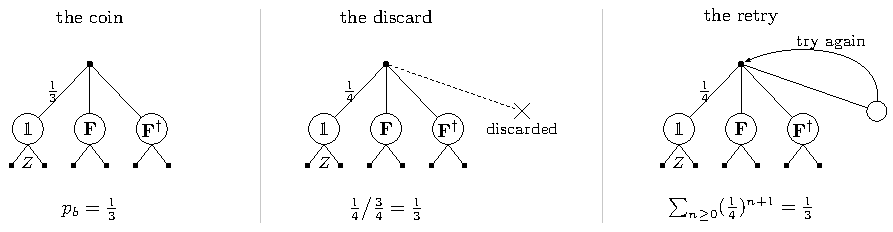
\includegraphics{../../paper/figures/protocol_doors.pdf}}{\fbox{\parbox{0.9\textwidth}{\centering\texttt{paper/figures/protocol\_doors.pdf} (the thesis's Figure~D.6) is not beside this file; the caption below describes it.}}}
\caption{The same door three times. Each panel is the octahedron's exhibition with one edge changed. The coin fans three ways and carries the $\tfrac{1}{3}$ as a bias; the discard fans four ways at dyadic weight $\tfrac{1}{4}$ and deletes the fourth branch, buying the same $\tfrac{1}{3}$ as a ratio of acceptance probabilities---one independent of the state, so the renormalization is legitimate; the retry keeps that branch and loops it, buying it as the limit of dyadic partial sums, at $\tfrac{4}{3}$ rounds expected. All three realize the six effects $\tfrac{1}{6}(\Id \pm \sigma_a)$ exactly, which is why \textit{deterministic} bans all three separately. Verified in \texttt{code/weight\_obstruction\_escapes.py}.}
\label{fig:protocol-doors}
\end{figure}

\subsection{The alignment corollary, slowly} \label{sec:decker:alignment}

The randomized-projective implementation (the thesis's Section~4.2.4) never needs the whole solid in one shot: each shot realizes one projective measurement along one drawn vertex, via an alignment rotation carrying $\hat v$ to $\hat z$ before the $Z$ readout. Could at least \textit{that} be exact, for some favorable vertex? No, and Corollary~\ref{cor:directions} already says so without a new idea. A projective measurement along $\hat v$ has two effects, $\tfrac{1}{2}(\Id \pm \hat v \cdot \sigmavec)$, and both are rank $1$---so the corollary applies to each and puts $\hat v$ itself in $K_\R^3$. Now the sweep (the thesis's Appendix~E.1, whose verdict \texttt{code/randomized\_implementations.py} confirms vertex-by-vertex): \textit{every} nonzero coordinate of a tetrahedron, cube, or dodecahedron vertex is $p/\sqrt{3}$ with $\abs{p} \in \{1, \invphig, \phig\}$, and of an icosahedron vertex $p/\sqrt{2+\phig}$ with $\abs{p} \in \{1, \phig\}$; both surds are barred by Lemma~\ref{lem:membership}, and the coset fact carries the bar to the quotients. No choice of vertex escapes; the projective route's field demand relocates into the alignment, it never dissolves.

The sweep has to be run and cannot be read off the witness: a single direction in isolation has no rotation invariant to fail, and can always be turned onto $\hat z$. What the sweep buys is therefore the atlas pose, where it bars \textit{every} vertex; pose-free, Lemma~\ref{lem:witness} still forbids a solid's vertices all lying in $K_\R^3$ together, so at least one drawn vertex fails however the solid is stood, and the projective route is never exact in any orientation. There is a second, narrower argument worth recording, because the thesis's Appendix~D.2 uses it. A circuit's Bloch rotation is a $K_\R$-matrix: its entries $R_{ab} = \tfrac12 \Tr[\sigma_a U \sigma_b U^\dagger]$ are sums of products of entries of $U$, their conjugates and Pauli entries---all in $K$---and each $R_{ab}$ is real, hence in $K_\R$. If $R\hat v = \hat z$ then $\hat v = R^\top \hat z$ is the third row of $R$, so an exactly-alignable vertex must be a $K_\R$-vector by that route too. The difference is what each assumes. The gate-level version assumes the alignment is a unitary on the data qubit, and says something about the gate; Corollary~\ref{cor:alignment} assumes only that the effects come out right, and says something about the protocol. The first is the finer statement, the second the stronger one.

What \textit{can} change is the route. Wherever the vertices pair antipodally, the randomized-projective coin realizes the same effects on a single qubit, with the atlas words of the thesis's Table~D.1 (\texttt{tab:decker-vs-coin}) in place of the ancilla register. The tetrahedron, indecomposable~\cite{dariano2005classicalrandomnessquantum}, is precisely where this exit is closed, and Decker's dilation stays the only route. Nor is the trade one gate for one: the dilation owes a second gate of another provenance, the reorientation of the thesis's Appendix~D.2---for the tetrahedron and the cube a $T^\dagger$, exact over Clifford${}+T$ and inexact over every gate set here without a $T$ in it---which the coin trades for the alignment. The thesis's Table~5.2 prices both routes.

\subsection{Where the bad numbers live}

The obstruction is geometric as well as arithmetic, and the dictionary is this thesis's own gate table read backwards. The offending coordinates sit on the rotation axes of the atlas gates: $F$'s axis pierces a tetrahedron, cube, and dodecahedron vertex, and its eigenstates are $T$-type magic states~\cite[Def.~1 and Fig.~1]{bravyi2005universalquantumcomputation}; $\Phi$'s axis is an icosahedron vertex, its eigenstates the antipodal pair there; $X$'s and $Z$'s axes are octahedron vertices, the stabilizer directions. In atlas orientation, a Platonic solid POVM is exactly implementable, never deterministically, if and only if its vertices are the Pauli axes; the other four point at magic states, whose non-constructibility by Clifford means is the resource-theoretic shadow of the same fact~\cite[Thm.~1 and \S3.2]{veitch2014resourcetheorystabilizer}.\footnote{Sharpest at the tetrahedron, whose fiducial \textit{is} the $T$-type magic state and maximizes the $p$-norm magic measure, for $p \in [1,2)$, over all qubit states~\cite[p.~1755]{feng2022stabilizerstatessicpovm}. That is a quantitative claim about distance from the stabilizer polytope where ours is a binary one about membership in a ring, and the two orderings do not coincide: $\ket{H}$ is magic and exactly preparable over Clifford${}+T$ all the same.} The refrain \textit{the measurement inherits the magic} is this section's arithmetic in one sentence: the field extensions that make magic states non-constructible by Clifford circuits are the ones the four inexact solids' vertices demand---and the exact solid is precisely the one whose vertices are the stabilizer axes themselves.

\begin{thebibliography}{99}
\bibitem{artin2011algebra} M.~Artin, \emph{Algebra}, 2nd ed., Pearson Education, Prentice Hall, 2011.
\bibitem{bravyi2005universalquantumcomputation} S.~Bravyi and A.~Kitaev, Universal quantum computation with ideal Clifford gates and noisy ancillas, \emph{Phys.\ Rev.\ A} \textbf{71}, 022316 (2005), \texttt{arXiv:quant-ph/0403025}.
\bibitem{dariano2005classicalrandomnessquantum} G.~M. D'Ariano, P.~Lo Presti and P.~Perinotti, Classical randomness in quantum measurements, \emph{J.\ Phys.\ A: Math.\ Gen.} \textbf{38}, 5979--5991 (2005).
\bibitem{feng2022stabilizerstatessicpovm} L.~Feng and S.~Luo, From stabilizer states to SIC-POVM fiducial states, \emph{Theor.\ Math.\ Phys.} \textbf{213}, 1747--1761 (2022).
\bibitem{ivashkov2024highfidelitymultiqubitgeneralized} P.~Ivashkov, G.~Uchehara, L.~Jiang, D.~S. Wang and A.~Seif, High-fidelity, multi-qubit generalized measurements with dynamic circuits, \emph{PRX Quantum} \textbf{5}, 030315 (2024), \texttt{arXiv:2312.14087}.
\bibitem{oszmaniec2017simulatingpositiveoperatorvaluedmeasures} M.~Oszmaniec, L.~Guerini, P.~Wittek and A.~Ac\'in, Simulating positive-operator-valued measures with projective measurements, \emph{Phys.\ Rev.\ Lett.} \textbf{119}, 190501 (2017), \texttt{arXiv:1609.06139}.
\bibitem{singal2022implementationquantummeasurements} T.~Singal, F.~B. Maciejewski and M.~Oszmaniec, Implementation of quantum measurements using classical resources and only a single ancillary qubit, \emph{npj Quantum Inf.} \textbf{8}, 82 (2022), \texttt{arXiv:2104.05612}.
\bibitem{veitch2014resourcetheorystabilizer} V.~Veitch, S.~A. H. Mousavian, D.~Gottesman and J.~Emerson, The resource theory of stabilizer computation, \emph{New J.\ Phys.} \textbf{16}, 013009 (2014), \texttt{arXiv:1307.7171}.
\bibitem{yordanov2019implementationgeneralsinglequbit} Y.~S. Yordanov and C.~H. W. Barnes, Implementation of a general single-qubit positive operator-valued measure on a circuit-based quantum computer, \emph{Phys.\ Rev.\ A} \textbf{100}, 062317 (2019), \texttt{arXiv:2001.04749}.
\end{thebibliography}

\end{document}
